%************************************************
\chapter{Auswahl des Kanalzugriffsverfahrens}\label{kap:zugriffsverfahren}
%************************************************

Nach dem zunächst kurz das ALOHA Protokoll als klassisches Kanalzugriffverfahren beschrieben wird, stellt dieses Kapitel zwei etablierte Verfahren im Detail vor.

\section{ALOHA}\label{kap:zugriffsverfahren_sec:aloha}
Als traditionelles Beispiel des Kanalzugriffes sei hier das \emph{ALOHA}-Protokoll aufgeführt. Kern des Verfahrens ist ein zufälliger Kanalzugriff der Netzwerkteilnehmer. Dabei wird davon ausgegangen, dass die Zwischenankunftszeit der gesendeten Pakete negativ exponentiell verteilt ist. Wird eine Kollision erkannt, wiederholt sich der Sendevorgang. In \autoref{fig:aloha} ist dieser Fall bei dem ersten bzw. zweiten Sendeversuch der Geräte A und B zu sehen. Die Geräte schließen auf eine Kollision, da nach einer bestimmten Zeit eine Bestätigung des Empfängers ausbleibt. Die Übertragung wird dann jeweils nach einer zufälligen Zeit wiederholt. Der maximale Durchsatz liegt dabei bei ca. 18 Prozent \citep{aloha}. 

\begin{figure}[bth]
        \myfloatalign
        {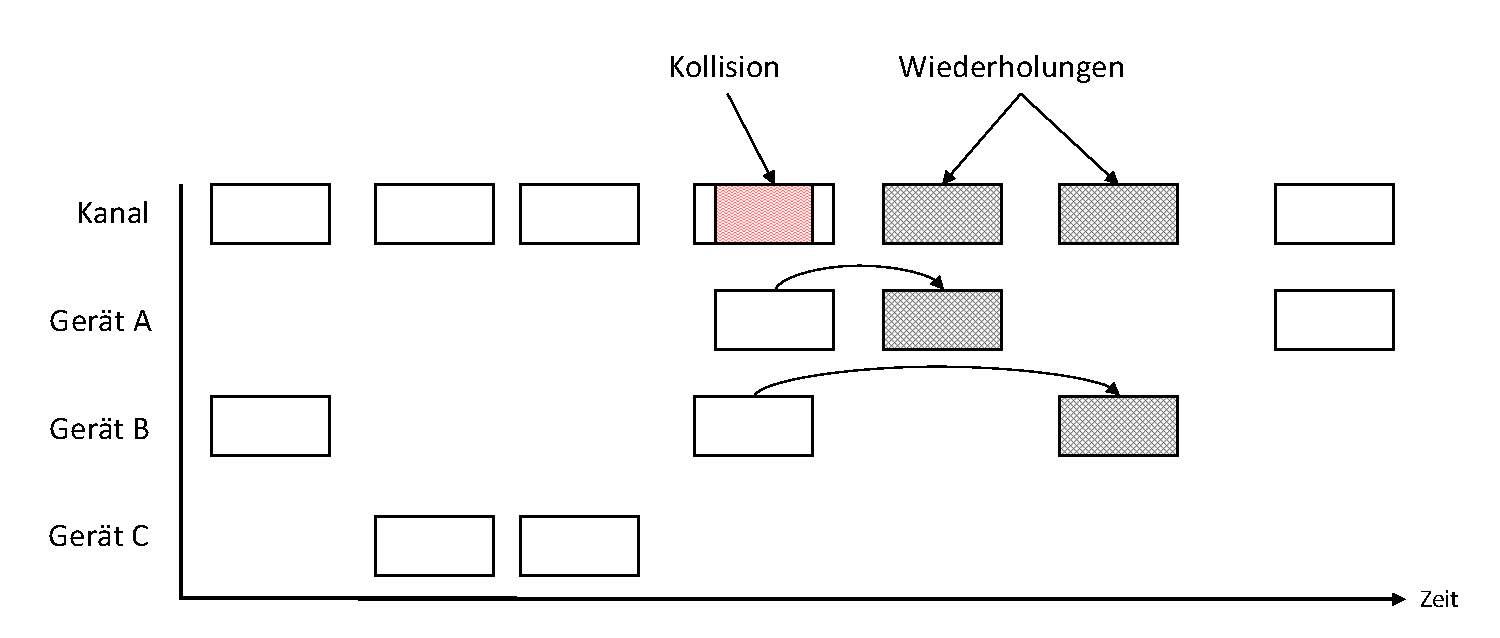
\includegraphics[width=1\linewidth]{gfx/ALOHA}} 
        \caption[ALOHA]{Beispiel für den Kanlazugriff nach dem ALOHA Protokoll }\label{fig:aloha}
\end{figure}

Die wiederholten Sendevorgänge wirken sich ungünstig auf den Energieverbrauch der \glspl{node} aus. Mit steigender Anzahl der Teilnehmer, wie es in Logistanwendungen der Fall ist, stößt dieses System an seine Grenzen \citep{inBinTestbed}. 

\section{Listen Before Talk}\label{kap:zugriffsverfahren_sec:lbt}
Das \emph{\ac{etsi}} befasst sich in \citep{lbt} mit der elektromagnetischen Verträglichkeit und der Nutzung des Funkspektrums durch \acp{srd}. Um die Ausnutzung des Funkkanals als begrenzte physikalische Ressource zu maximieren, beschreibt dieser Standard einen \ac{lbt} Kanalzugriff. 

Ist ein Gerät im Begriff, eine Übertragung zu starten, soll es zunächst den Funkkanal nach Aktivitäten anderer Geräte abhören und die eigentliche Übertragung noch zurückhalten. Die Abhörzeit $t_{\textrm{L}}$ setzt sich aus einer festen und einer zufälligen Komponente zusammen:
\begin{equation}
{t_{\textrm{L}}} = {t_{\textrm{F}}} + {t_{\textrm{PS}}}
\end{equation}
${t_{\textrm{F}}}$ beträgt $5ms$, während ${t_{\textrm{PS}}}$ einen zufälligen Wert zwischen $0ms$ und $5ms$ annimmt. Wird innerhalb von ${t_{\textrm{F}}}$ keine Aktivität erkannt, beginnt der Sendevorgang direkt im Anschluss und ${t_{\textrm{PS}}}$ wird zu $0$ gesetzt. Wohingegen im Fall eines belegten Kanals die Abhörzeit unterbrochen wird bis der Kanal wieder frei ist. Im Anschluss wird der Kanal für die gesamte Dauer von ${t_{\textrm{L}}}$ abgehört, die durch den Anteil von ${t_{\textrm{PS}}}$ variieren kann. \autoref{fig:lbt} verdeutlicht diese Verfahren exemplarisch für drei Geräte. \texttt{Gerät C} detektiert keine Aktivität auf dem Kanal innerhalb der $5ms$ Abhörzeit und startet daher unverzüglich mit der Übertragung. \texttt{Gerät B} und \texttt{Gerät A}, die zu diesem Zeitpunkt jeweils eine Übertragung ausstehen haben, können diese erst nach zwei bzw. drei Abhörzyklen beginnen.

In \autoref{fig:lbt} wird auch deutlich, wann sich die Geräte im Sende- , bzw. Empfangsmodus befinden. Um den Kanal abzuhören, muss sich ein Gerät im Empfangsmodus befinden. Der \ac{lbt} Algorithmus sieht vor, dass im Fall eines belegten Kanals solange gewartet wird, bis dieser wieder frei ist. Auch in dieser Zeit muss ein Gerät im Empfangsstatus verbleiben, um den Zeitpunkt festzustellen, wann der Kanal wieder frei ist und der Backoff-Mechanismus erneut gestartet werden kann. Im Vergleich zu \texttt{Gerät C} ergibt sich für \texttt{Gerät A} eine erheblich längere Zeitspanne im Empfangsmodus.

\begin{figure}[bth]
        \myfloatalign
        {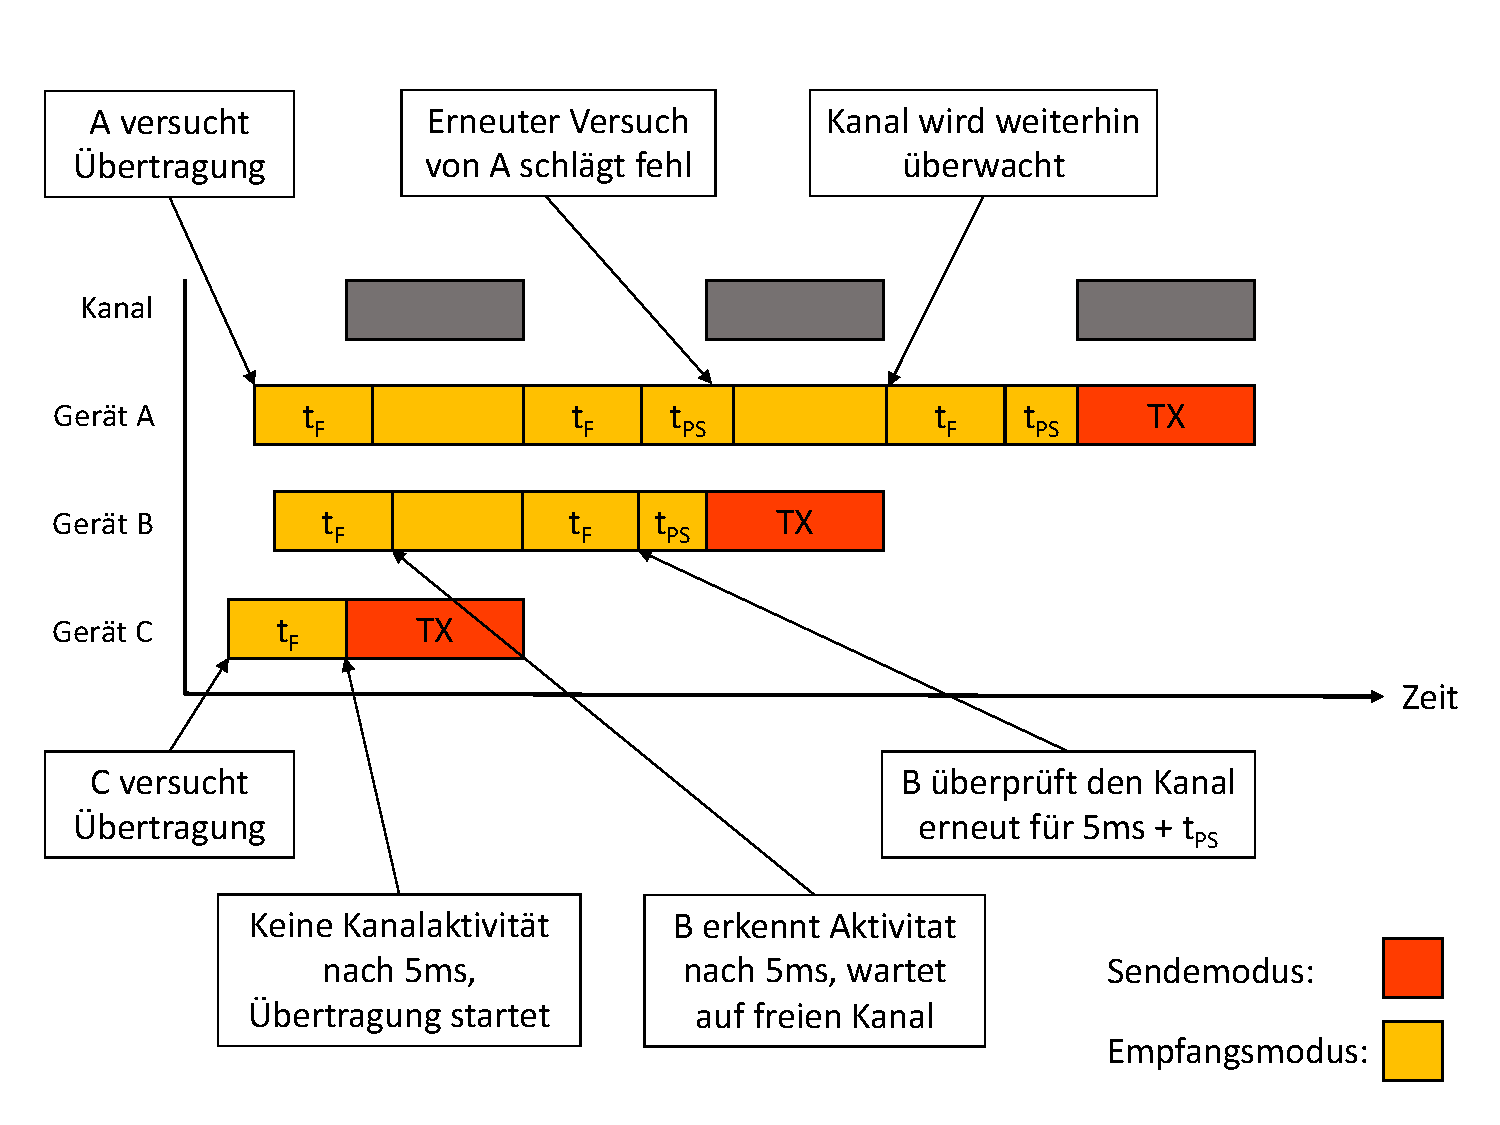
\includegraphics[width=1\linewidth]{gfx/LBT}} 
        \caption[Listen Before Talk]{Beispiel für den LBT Algorithmus bei drei konkurrierenden Kanalzugriffen. Die orange markierten Zeiten repräsentieren Empfangsstatus, die roten Sendestatus.}\label{fig:lbt}
\end{figure}

\section{Carrier Sense Multiple Access / Collision Avoidance}\label{kap:zugriffsverfahren_sec:csma}
Das \ac{ieee} standardisiert in \cite{ieee} die Bitübertragung (\emph{Physical Layer}) und den Kanalzugriff (\acs{mac}-\emph{Layer}) als Teil der Verbindungssicherung\footnote{im Bezug auf das \acl{osi} Referenzmodell der \acs{iso}} für Sensornetzwerke mit niedriger Datenrate. Das Protokoll sieht vor, dass vor Beginn einer Übertragung ein \acl{csma} Algorithmus durchlaufen wird. Ähnlich dem \acs{lbt} sieht dieser vor, eine Übertragung zunächst nach einem bestimmten Muster zurückzuhalten. Dieser Vorgang wird \emph{Backoff} genannt. In der Grundversion muss ein Gerät zwei Variablen zur Durchführung des Algorithmus verwalten:
\begin{enumerate}
	\item $NB$: Anzahl der Durchläufe des Algorithmus für den aktuellen Sendeversuch
	\item $BE$: Backoff-Exponent, der den Backoff-Zeitraum eingrenzt
\end{enumerate}
Alle Zeitangaben, die in dem Standard beschrieben werden, beziehen sich auf die Übertragungsdauer eines Symbols, die \emph{Symbol Period}. Dem \acs{csma} Verfahren liegt der Einheitszeitraum \emph{Unit Backoff Period} zugrunde, der aus 20 \emph{Symbol Periods} besteht \cite{ieee}. Mit den in dieser Arbeit gewählten Einstellungen\footnote{Symbolrate = $20 \frac{kSymbols}{s}$, (Bitrate = $20 \frac{kBit}{s}$, BPSK Modulation)} ergibt sich:
\begin{center}
\emph{Unit Backoff Period} $ = 1ms$
\end{center}
Die Backoff-Zeiten sind ganzzahlige Vielfache dieses Zeitraums und  werden zufällig bestimmt. Die Menge der möglichen Werte ist: 
\begin{center}
$\{0, (2\textsuperscript{BE})-1)\}$  \emph{Unit Backoff Periods}
\end{center}
Die Variable $BE$ begrenzt somit die Auswahl der möglichen Backoff-Zeiten. Ein Blockdiagramm des Algorithmus ist in \autoref{ahg:csmablock} zu sehen. In \autoref{fig:csma} ist das Verfahren exemplarisch mit drei konkurrierenden Sendeversuchen dargestellt. Jedes Gerät hält seine Übertragung zunächst für eine zufällige Zeit, wie zuvor beschrieben, zurück. Im Anschluss wird die Aktivität auf dem Funkkanal überprüft (\acf{cca}). Die Prüfung des Kanals soll nach \citep{ieee} $0,4ms$ dauern. In \autoref{fig:csma} stellt Gerät B nach der Kanalprüfung keine Aktivität fest und beginnt mit dem Sendevorgang. Für dieses Gerät hat der Algorithmus an dieser Stelle erfolgreich terminiert. Die Kanalprüfung der Geräte A und C fällt negativ aus, sodass der Algorithmus die nächste Iteration durchläuft. Dabei werden nun die Variablen $NB$ und $BE$ jeweils um eins erhöht, wie \autoref{ahg:csmablock} zu entnehmen ist. Dadurch steigt die Anzahl der möglichen Backoff-Zeiten mit jedem Durchlauf. Dies bedeutet nicht, dass die konkreten Backoff-Zeiten stetig größer werden, es stehen nur mehrere verschiedene Zeiträume zur Verfügung.
Anzumerken ist, dass sich die Geräte während des Backoffs nicht im Empfangsstatus befinden müssen. 

\begin{figure}[bth]
        \myfloatalign
        {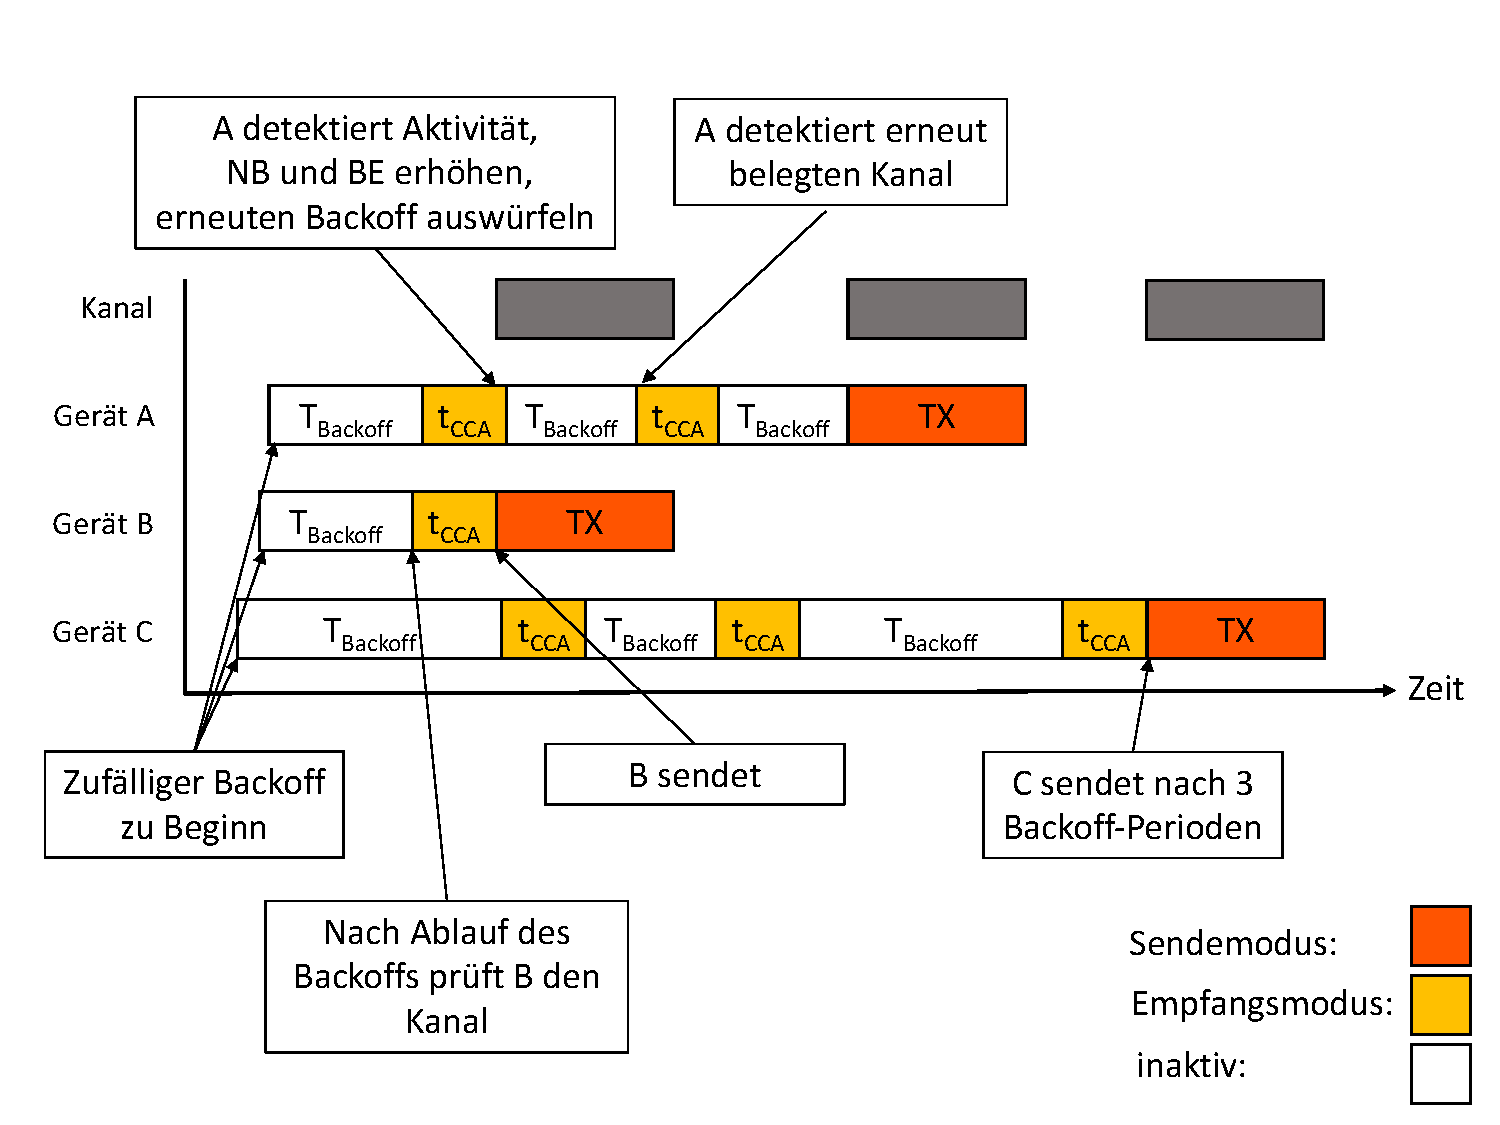
\includegraphics[width=1\linewidth]{gfx/CSMA}} 
        \caption[Carrier Sense Multiple Access]{Beispiel für den CSMA-CA Algorithmus bei drei konkurrierenden Kanalzuriffen. Die orange markierten Zeiten repräsentieren Empfangsmodus, die roten Sendemodus. Während der weiß markierten Zeiten ist kein aktiver Modus notwendig. }\label{fig:csma}
\end{figure}

\section{Schlussfolgerung für die weitere Untersuchung}

Ein unkoordinierter Kanalzugriff nach dem ALOHA Ansatz führt bei einer großen Teilnehmeranzahl zu vielen Kollisionen. Übertragungen müssen dann wiederholt werden, was sich negativ auf den Energieverbrauch auswirkt. Dieser Ansatz ist daher für den Einsatz in einem großskaligen \acs{wsn} mit stark eingeschränkter Energieverfügbarkeit der \glspl{node} nicht geeignet \cite{inBinTestbed}. 

Die eine genaue Untersuchung des \acs{lbt} und des \acs{csma} Verfahrens sind dagegen in Erwägung zu ziehen \cite{Falkenberg2017b}\citep{GreenOrbs}. Im Vergleich von \autoref{fig:lbt} und \autoref{fig:csma} wird jedoch deutlich, dass der \acs{csma} Algorithmus hinsichtlich der Energieeffizienz deutliche Vorteile aufweist. Der dramatische Anstieg des mittleren Energieverbrauchs pro \gls{node} bei Verwendung von \acs{lbt} wird in \citep{Falkenberg2017b} demonstriert.
Daher wird im Folgenden das \acs{csma} Zugriffsverfahren nach dem \gls{802154} Standard näher untersucht. 

%*****************************************
%*****************************************
%*****************************************
%*****************************************
%*****************************************




